\documentclass[fleqn]{MJD}

\usepackage{cancel}
\usepackage{cleveref}
\usepackage{titlesec}
\usepackage{hyperref}
%\colorsections
%\bluelinks
\newcommand{\problem}[1]{\chapter{Problem #1}}
\newcommand{\subproblem}[2]{\section{(#1)~ #2}}
\newcommand{\subsubproblem}[2]{\subsection{ #1)~ #2}}
\newcommand{\U}{\cup}
\renewcommand{\S}{\mathcal{S}}
\renewcommand{\s}{\subset}
\renewcommand{\equiv}{\Leftrightarrow}
\newcommand{\0}{\emptyset}
\newcommand{\imp}{\Rightarrow}
\newcommand{\Usum}{\bigcup\limits_{i=1}^\infty}
\newcommand{\intsum}{\bigcup\limits_{i=1}^\infty}
\newcommand{\infsum}{\sum\limits_{i=1}^\infty}
\newcommand{\sets}{\{A_1, A_2 \dots\} }
\newcommand{\nsets}{\{A_1, \dots, A_n \} }

\titleformat{\chapter}[display]
  {\normalfont\bfseries}{}{0pt}{\LARGE}
  
\graphicspath{ {../} }

%%%%%%%%%%%%%%%%%%%%%%%%%%%%%%%%%%%%
\begin{document}
\lstset{language=Python}
\titleAT[CS 224N: Assignment 2]{Peter888@stanford.edu}
%-------------------------------------
\problem{1: Tensorflow Softmax (25 points)}
%-------------------------------------

%----------------------
\subproblem{a}{Implement Softmax use Tensorflow (5 points, coding)}
\noindent\textbf{Answer:} \\
\noindent See code: $\sim$\verb|/q1_softmax.py|.

\vskip3em

%----------------------
\subproblem{b}{Implement Cross-Entropy use Tensorflow (5 points, coding)}
\noindent \textbf{Answer:} \\

\noindent See code: $\sim$\verb|/q1_softmax.py|.

\vskip3em
%----------------------
\subproblem{c}{Tensorflow Placeholder and Feed Dictionary (5 points, coding/written)}
\noindent \textbf{Answer:} \\
\noindent See code: $\sim$\verb|/q1_classifier.py|.  \\ \\
\noindent \textit {Explanation:} \\
\indent \textit{Placeholder variables and feed dictionary make it possible to feed external data (such as training data for network) into Tensorflow's computational graph.}
\vskip3em

%----------------------
\subproblem{d}{Implement Classifier (5 points, coding)}
\noindent\textbf{Answer:} \\
\noindent See code: $\sim$\verb|/q1_classifier.py|.

\vskip3em
%----------------------
\subproblem{e}{Implement Model (5 points, coding/written)}
\noindent\textbf{Answer:} \\
\noindent See code: $\sim$\verb|/q1_classifier.py|. \\ \\
\noindent \textit {Explanation:} \\
\indent \textit {When the model's $train\_op$ is called. Computation going forward through the computation graph with Placeholder's input and the init/start values in Variables. The Tensorflow automatic differentiation will start the backward propagation, it will automatically calculate the gradients and differentiations, and update the Variables back through the computation graph.}
\vskip3em
\newpage
%-------------------------------------
\problem{2: Neural Transition-Based Dependency Parsing (50 points + 2 bonus points)}
%-------------------------------------

%----------------------
\subproblem{a}{Dependency Parsing (6 points, written)}

\noindent \textbf{Answer:}


\begin{table}[!htbp]
	\centering
	\small
\begin{tabular}{l|l|l|l}
\textbf{stack} 						& \textbf{buffer}							& \textbf{ new dependency}	& \textbf{transition} 	\\ \hline 
$[ROOT]$ 							& $[I, parsed, this, sentence, correctly]$  &  							& Initial Configuration \\ 
$[ROOT, I]$ 						& $[parsed, this, sentence, correctly]$ 	&  							& \verb|SHIFT|  		\\ 
$[ROOT, I, parsed]$ 				& $[this, sentence, correctly]$ 			&  							& \verb|SHIFT|  		\\ 
$[ROOT, parsed]$ 					& $[this, sentence, correctly]$ 			& parsed $\rightarrow$ I 	& \verb|LEFT-ARC| 		\\ \hline
$[ROOT, parsed, this]$				& $[sentence, correctly]$ 					&  							& \verb|SHIFT|  		\\ 
$[ROOT, parsed, this, sentence]$	& $[correctly]$ 							&   						& \verb|SHIFT| 			\\ 
$[ROOT, parsed, sentence]$ 			& $[correctly]$ 						& sentence $\rightarrow$ this	& \verb|LEFT-ARC| 		\\ 
$[ROOT, parsed]$ 					& $[correctly]$ 						& parsed $\rightarrow$ sentence	& \verb|RIGHT-ARC| 		\\ 
$[ROOT, parsed, correctly]$			& $[ ]$ 									&   						& \verb|SHIFT| 			\\ 
$[ROOT, parsed]$ 					& $[ ]$ 								& parsed $\rightarrow$ correctly& \verb|RIGHT-ARC| 		\\ 
$[ROOT]$ 							& $[ ]$ 									& ROOT $\rightarrow$ parsed & \verb|RIGHT-ARC| 		\\
\end{tabular} 
\end{table}



%----------------------
\subproblem{b}{How many steps (2 points, written)}
\label{prob:2b}
\noindent \textbf{Answer:} 

\textit {$2n$ parse steps. Because each word take exactly one shift transition from buffer to stack, take exactly one *-ARC (either LEFT-ARC or RIGHT-ARC) transition move out from stack, and every transition either add or remove word in the stack.}

\vskip4em


\subproblem{c}{Parser Step (6 points, coding)}

\noindent See code: $\sim$\verb|/q2_parser_transitions.py|.
\vskip4em
%----------------------
\subproblem{d}{Parser Transitions (6 points, coding)}

\noindent See code: $\sim$\verb|/q2_parser_transitions.py|.
\vskip4em
%----------------------

\subproblem{e}{Xavier Initialization (4 points, coding)}

\noindent See code: $\sim$\verb|/q2_initialization.py|.

%----------------------
\subproblem{f}{Dropout (2 points, written)}
\noindent \textbf{Answer:}  \\
\begin{align}
 \gamma = \frac{1}{1-p_{drop}} \nonumber
 \end{align}
 \indent \textit{The mask vector $\bm{d}$ set entries in $\bm{h}$ to zero at probability $p_{drop} $, let's say $\bm{h}$ has full expectation value $\mathbb{E}[\bm{h}]$=1, so $\mathbb{E}[\bm{d} \circ \bm{h}]$=(1-$p_{drop}$), this because $p_{drop}$ of $\bm{h}$ values are become zero. \\ \\
 %
 \indent So, $1 = \frac{\mathbb{E}[\bm{d} \circ \bm{h}]}{(1-p_{drop})} \Rightarrow 1=\mathbb{E}[\bm{h}_{drop}]=\frac{1}{(1-p_{drop})}\mathbb{E}[\bm{d} \circ \bm{h}] \Rightarrow \gamma = \frac{1}{1-p_{drop}}$ }
\vskip4em

%----------------------
\subproblem{g}{Adam Optimizer (4 points, written)}
\subsubproblem{i}{Momentum}
\noindent \textbf{Answer:} \\
\indent \textit{The rolling average, $m$, can reduce the variance in updates, by down-weighting the impact of the current minibatch's gradient. For instance, if $\beta$ is 0.5, when updating $\bm{\theta}$, it will use half of past rolling average $m$, and half of current minibatch's gradient. Consider if the current minibatch's gradient varies too larger or too smaller than the last rolling average $m$, the momentum will reduce the larger or smaller part of the gradient to just half to get new $m$, and use the reduced new $m$ to do update. }
\vskip4em
\subsubproblem{ii}{Adaptive Learning Rates}
\noindent \textbf{Answer:} \\
\indent \textit {The parameters with smaller gradients (especial rolling average smaller) will get larger updates. For parameters been changing flatly, the adaptive learning rate will help to these parameter get larger updates, and helping these parameter move off plateaus. This can increase learning speed.}
\vskip4em

%----------------------
\subproblem{h}{Parser Model (20 points, coding/written)}
\noindent \textbf{Answer:} 
\noindent \\ See code: $\sim$\verb|/q2_parser_model.py|. \\
\indent \textit{Report the best UAS} \\
\indent \textit {
The best dev UAS: 88.11,  and it's test UAS: 88.31 \\
}
\indent \textit{List of predicted labels, see file $q2\_test.predicted.pkl$} \\

\vskip4em

%----------------------
\subproblem{i}{Bonus (2 points, coding/written)}
\noindent \textbf{Answer: } \\
\indent \textit{Implemented L2 regularization. The best dev UAS: 87.49, and it's test UAS: 87.86. There is no significant improvement by using L2 regularization. This could be the overfit not due to parameters values, need to tune other hyper-parameters such as hidden layer size, or dropout rate.} 
\vskip4em

\newpage
%-------------------------------------
\problem{3: Recurrent Neural Networks (25 points + 1 bonus point)}
%-------------------------------------

%----------------------
\subproblem{a}{ Perplexity (4 points, written)}
\subsubproblem{i} {Derive Perplexity (2 points)}
\noindent \textbf{Answer:} \\ \\
\textit {  As $\bm{y^{(t)}}$ is an one-hot vector, assume the k-th element $y_{k}^{(t)}$ is 1 \\ \\
so, }\\ 
\begin{align} \bm{J}^{(t)}(\bm{\theta})=-log(\hat{y}_{k}^{(t)})=log(\frac{1}{\hat{y}_{k}^{(t)}})
\end{align}
\textit{and we also have }\\ 
\begin{align} 
PP^{(t)}(\bm{y}^{(t)},\bm{\hat{y}}^{(t)})=\frac{1}{\hat{y}_{k}^{(t)}}
\end{align}
\textit{thus, we have }\\ 
\begin{align}
\bm{J}^{(t)}(\bm{\theta})=log(PP^{(t)}(\bm{y}^{(t)},\bm{\hat{y}}^{(t)}))
\end{align}

\vskip2em
\subsubproblem{ii} {Equivalent (1 point)}
\noindent \textbf{Answer:} \\
\textit {
We know $min\{log(f(x)\}=min\{f(x)\}, f(x)>0$ \\ \\
then we have, }\\
\begin{align}
min\{\bm{J}^{(t)}(\bm{\theta})=log(PP(\bm{y}^{(t)},\bm{\hat{y}}^{(t)})):\bm{\theta}>0\}=min\{PP^{(t)}(\bm{y}^{(t)},\bm{\hat{y}}^{(t)})\} \forall (t \in [1..T]) \nonumber
\end{align}
\textit {from convex theory not hard to know minimizing the geometric mean equivalent to minimizing the arithmetic mean if the related function have same minimizing equivalent. }\\ \\
\indent \textit {
$min\{(\prod_{j=1}^{T}f_{j}(x))^{\frac{1}{T}}\}=min\{\frac{1}{T}\sum_{i=1}^{T}(g_{i}(x))\}$, when $min\{\bm{f}(x)\}=min\{\bm{g}(x)\}$, for $\bm{f}$,$\bm{g}$ are positive functions\\ \\
Finally, we can get the minimizing geometric mean perplexity equivalent to minimizing the arithmetic mean cross-entropy loss \\ \\
$\indent$ $min\{(\prod_{t=1}^{T}PP(\bm{y}^{(t)},\bm{\hat{y}}^{(t)}))^{\frac{1}{T}}\}$ = $min\{\frac{1}{T}\sum_{t=1}^{T}CE(\bm{y}^{(t)},\bm{\hat{y}}^{(t)})\}$\\ \\
}
\vskip2em
\newpage
\subsubproblem{iii} {Perplexity for a single word (1 point)}
\noindent \textbf{Answer:} \\
\textit {
for given word $\bm{\omega}_j$, \\ \\
$\indent$ $\bar{P} \left( \bm{x}^{(t+1)} = \bm{\omega}_j \vert \bm{x}^{(t)}, \dots, \bm{x }^{(1)} \right)=\frac{1}{\vert V \vert}$  \\ \\
so the perplexity for that single word $\bm{\omega}_j$, is $\vert V \vert$\\ \\
$\indent$$PP^{(t)}(\bm{y}^{(t)},\bm{\hat{y}}^{(t)}=1/\frac{1}{\vert V \vert} = \vert V \vert$ \\ \\
because, $\bm{J}^{(t)}(\bm{\theta})=log(PP^{(t)}(\bm{y}^{(t)},\bm{\hat{y}}^{(t)}))$, when $\vert V \vert$=10000 \\ \\
$\indent$$\bm{J}^{(t)}(\bm{\theta})=log(\vert V \vert) \approx 9.213$
}
\vskip2em

%----------------------
\subproblem{b}{Gradients on Single Point (7 points, written)}

\noindent \textbf{Answer:} 

\begin{align}
	\bm{\delta_{1}^{(t)}} &= \frac{\partial{\bm{J}}}{\partial{\bm{\theta}}^{(t)}} = -\mathbf{y} + \hat{\mathbf{y}}  
\end{align}
\textit{Write sigmoid(x) as $\sigma(x)$, and it's derivative as $\sigma^{'}(x)$}
\begin{align}
	\bm{\delta_{2}^{(t)}} &= \frac{\partial{\bm{J}}}{\partial{\bm{z}}^{(t)}} = \bm{\delta_{1}^{(t)}} \frac{\partial{\bm{\theta}^{(t)}}}{\partial{\bm{h}}^{(t)}}  \frac{\partial{\bm{h}}^{(t)}}{\partial{\bm{z}}^{(t)}}  \nonumber \\%
	&=\bm{U}^{T} \cdot \bm{\delta_{1}^{(t)}} \circ \sigma^{'}(\bm{z}^{(t)})  \nonumber \\
	&=\bm{U}^{T} \cdot \bm{\delta_{1}^{(t)}} \circ \bm{h}^{(t)} \circ (1 -  \bm{h}^{(t)})  \\
	 \frac{\partial{\bm{J}^{(t)}}}{\partial{\bm{U}}} &= \frac{\partial{\bm{J}^{(t)}}}{\partial{\bm{\theta}}^{(t)}}  \frac{\partial{\bm{\theta}^{(t)}}}{\partial{\bm{U}}} %
	 = \bm{\delta_{1}^{(t)}} (\bm{h}^{(t)})^{T}  \\
	 \frac{\partial{\bm{J}^{(t)}}}{\partial{\bm{e}^{(t)}}} &= \frac{\partial{\bm{J}^{(t)}}}{\partial{\bm{z}^{(t)}}} \frac{\partial{\bm{z}^{(t)}}}{\partial{\bm{e}^{(t)}}} %
	 =  (\bm{W}_{e} \vert_{(t)})^{T} \bm{\delta_{2}^{(t)}}  \\
	 \frac{\partial{\bm{J}^{(t)}}}{\partial{\bm{W_{e}}}} \bigg\rvert_{(t)} &=\frac{\partial{\bm{J}^{(t)}}}{\partial{\bm{z}^{(t)}}}  \frac{\partial{\bm{z}^{(t)}}}{\partial{\bm{W_{e}}}} \bigg\rvert_{(t)} %
	 = \bm{\delta_{2}^{(t)}} (\bm{e}^{(t)})^{T}  \\
	 \frac{\partial{\bm{J}^{(t)}}}{\partial{\bm{W}_{h}}}  \bigg\rvert_{(t)} &= \frac{\partial{\bm{J}^{(t)}}}{\partial{\bm{z}}^{(t)}}  \frac{\partial{\bm{z}^{(t)}}}{\partial{\bm{W}_{h}}} \bigg\rvert_{(t)} %
	 =  \bm{\delta_{2}^{(t)}} (\bm{h}^{(t-1)})^{T}  \\
	 \frac{\partial{\bm{J}^{(t)}}}{\partial{\bm{h}^{(t-1)}}} &= \frac{\partial{\bm{J}^{(t)}}}{\partial{\bm{z}^{(t)}}} \frac{\partial{\bm{z}^{(t)}}}{\partial{\bm{h}^{(t-1)}}} %
	 =  (\bm{W}_{h} \vert_{(t)})^{T} \bm{\delta_{2}^{(t)}}  
\end{align}

\vskip5em

\newpage
%----------------------
\subproblem{c}{Gradients (7 points, written)}
\noindent \textbf{Answer:} \\
\begin{figure}[!htbp]
	\caption{Unrolled RNN}
	\label{figure:unrolled3timesteps}
	\centering
	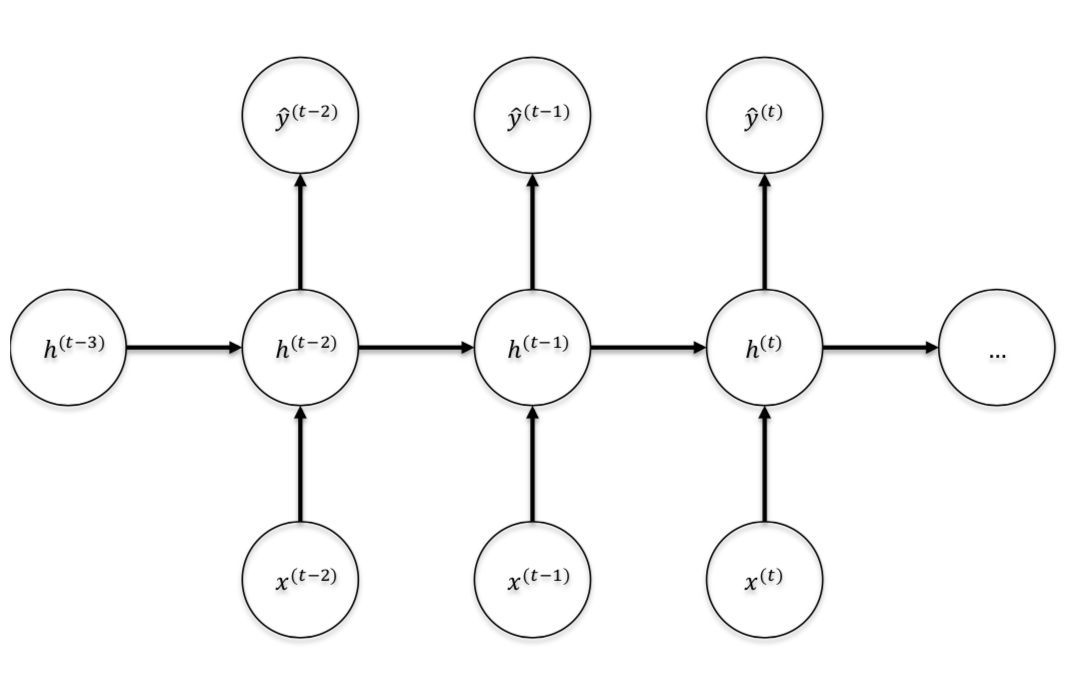
\includegraphics[scale=0.75]{unrolled3timesteps}
\end{figure}
\textit {} \\
\textit {We know:} 
\begin{align}
\bm{z}^{(t-1)}&=\bm{W}_{h} \vert_{(t-1)} \bm{h}^{(t-2)} + \bm{W}_{e} \vert_{(t-1)} \bm{e}^{(t-1)} + \bm{b}_{1}\vert_{(t-1)}\\
\bm{h}^{(t-1)}&= sigmoid(\bm{z}^{(t-1)})=\sigma({\bm{z}}^{(t-1)}) \\
\bm{\gamma}^{(t-1)} &= \frac{\partial{\bm{J}^{(t)}}}{\partial{\bm{h}^{(t-1)}}} 
\end{align}
\textit {Then,} \\
\begin{align}
\bm{\delta_{2}^{(t-1)}} &= \frac{\partial{\bm{J}}^{(t)}}{\partial{\bm{z}}^{(t-1)}} = \frac{\partial{\bm{J}^{(t)}}}{\partial{\bm{h}^{(t-1)}}} % 
	\frac{\partial{\bm{h}}^{(t-1)}}{\partial{\bm{z}}^{(t-1)}}  \nonumber \\
	&=\bm{\gamma}^{(t-1)}  \circ \sigma^{'}(\bm{z}^{(t-1)})  \nonumber \\
	&=\bm{\gamma}^{(t-1)}  \circ \bm{h}^{(t-1)} \circ (1 - \bm{h}^{(t-1)}) \\ 
\frac{\partial{\bm{J}^{(t)}}}{\partial{\bm{e}^{(t-1)}}} &= \frac{\partial{\bm{J}^{(t)}}}{\partial{\bm{z}^{(t-1)}}}  %
		\frac{\partial{\bm{z}^{(t-1)}}}{\partial{\bm{e}^{(t-1)}}} %
	 =  (\bm{W}_{e} \vert_{(t-1)})^{T} \bm{\delta_{2}^{(t-1)}}  \\
	 \frac{\partial{\bm{J}^{(t)}}}{\partial{\bm{W_{e}}}} \bigg\rvert_{(t-1)} &=\frac{\partial{\bm{J}^{(t)}}}{\partial{\bm{z}^{(t-1)}}}  %
	 		\frac{\partial{\bm{z}^{(t-1)}}}{\partial{\bm{W_{e}}}} \bigg\rvert_{(t-1)} %
	 = \bm{\delta_{2}^{(t-1)}} (\bm{e}^{(t-1)})^{T}  \\
	 \frac{\partial{\bm{J}^{(t)}}}{\partial{\bm{W}_{h}}}  \bigg\rvert_{(t-1)} &= \frac{\partial{\bm{J}^{(t)}}}{\partial{\bm{z}}^{(t-1)}} %
	 		 \frac{\partial{\bm{z}^{(t-1)}}}{\partial{\bm{W}_{h}}} \bigg\rvert_{(t-1)} %
	 =  \bm{\delta_{2}^{(t-1)}} (\bm{h}^{(t-2)})^{T}  
\end{align}
\vskip5em
\newpage
%----------------------
\subproblem{d}{How Many Operations for Single Timestep (3 points, written)}
\noindent \textbf{Answer:} \\
\indent \textit {Go through each equations in part (b), those backpropagation's operations are $O(|V| \times D_{h})$,  $O(d \times D_{h})$ and  $O(D_{h} \times D_{h})$, adding up all those operations, for a single step the operation count is $\bm{O}(|V| \times D_h + d \times D_h + D_h \times D_h)$} 
%----------------------
\subproblem{e}{How Many Operations for Entire Sequence (3 points, written)}

\noindent \textbf{Answer:}  \\
\indent \textit {Go through each backpropagation equations operation in part (c), the operation count also $\bm{O}(|V| \times D_h + d \times D_h + D_h \times D_h)$.  So for T words, the total operation count is $\bm{O}(T \times (|V| \times D_h + d \times D_h + D_h \times D_h))$}

%----------------------
\subproblem{f}{Which largest? Term RNN? (1 point, written)}

\noindent \textbf{Answer:}  \\
\indent \textit {$\bm{O}(|V| \times D_h)$ term is the largest. Word dictionary $|V|$is normally large, and $D_h << |V|$. It happens when backpropagate from output layer to hidden layer.}

%----------------------
\subproblem{g}{Bonus (1 point, written)}
\noindent \textbf{Answer:} \\
\textit {If we can change the operation count from  $\bm{O}(T \times (|V| \times D_h + d \times D_h + D_h \times D_h))$ to  $\bm{O}(T \times (C \times D_h + d \times D_h + D_h \times D_h))$, by mapping words to classes, and C  is the number of classes, because $C<|V|$, this will speed up the calculation. And this approach suggested by the paper "Externsions of recurrent neural network language model" (Mikolov, et al. 2013) 
}

\end{document}
